\subsection{Product perspective}
Domande utili per UML:
\begin{enumerate}
      \item C'è una relazione 1:1 tra CPO e CPMS oppure un CPO è una compagnia che gestisce tante stazioni di ricarica?
            \\ Per ogni CPO c'è un CPMS che amministra PIÙ stazioni di ricarica
      \item Mi immagino il CPMS come una periferica che ha ogni stazione a disposizione, l'UML mostra la struttura dati / funzionale del sistema eMSP, quindi non ha la facoltà di aggiornare attivamente i componenti come CPMS e socket. Vogliamo includere un'interfaccia che permetta a questi componenti di fare una richiesta al server per aggiornare i dati?\\
            Per quanto riguarda l'utilizzare un'altra interfaccia pensavo di inserire un'interfaccia che permettesse di interfacciarsi con il CPMS e con i vari sockets del modello centralizzato. In questo modo non si intaccherebbe l'interfaccia utente e ci sarebbe modo di avere un "filo" di ragionamento coerente con il modello e con la rappresentazione fisica.
      \item Il pattern più comodo per il sistema sarebbe partire sempre da una richiesta del client e poi rispondere. Mi chiedo quindi se è possibile seguire questo profilo in tutto il progetto. Per il calendario pensavo che il client (leggermente fat) potesse chiedere ogni tot al server se sarebbe un buon momento per fare rifornimento ed il server risponde.
\end{enumerate}
\begin{figure}[h!]
      \begin{center}
            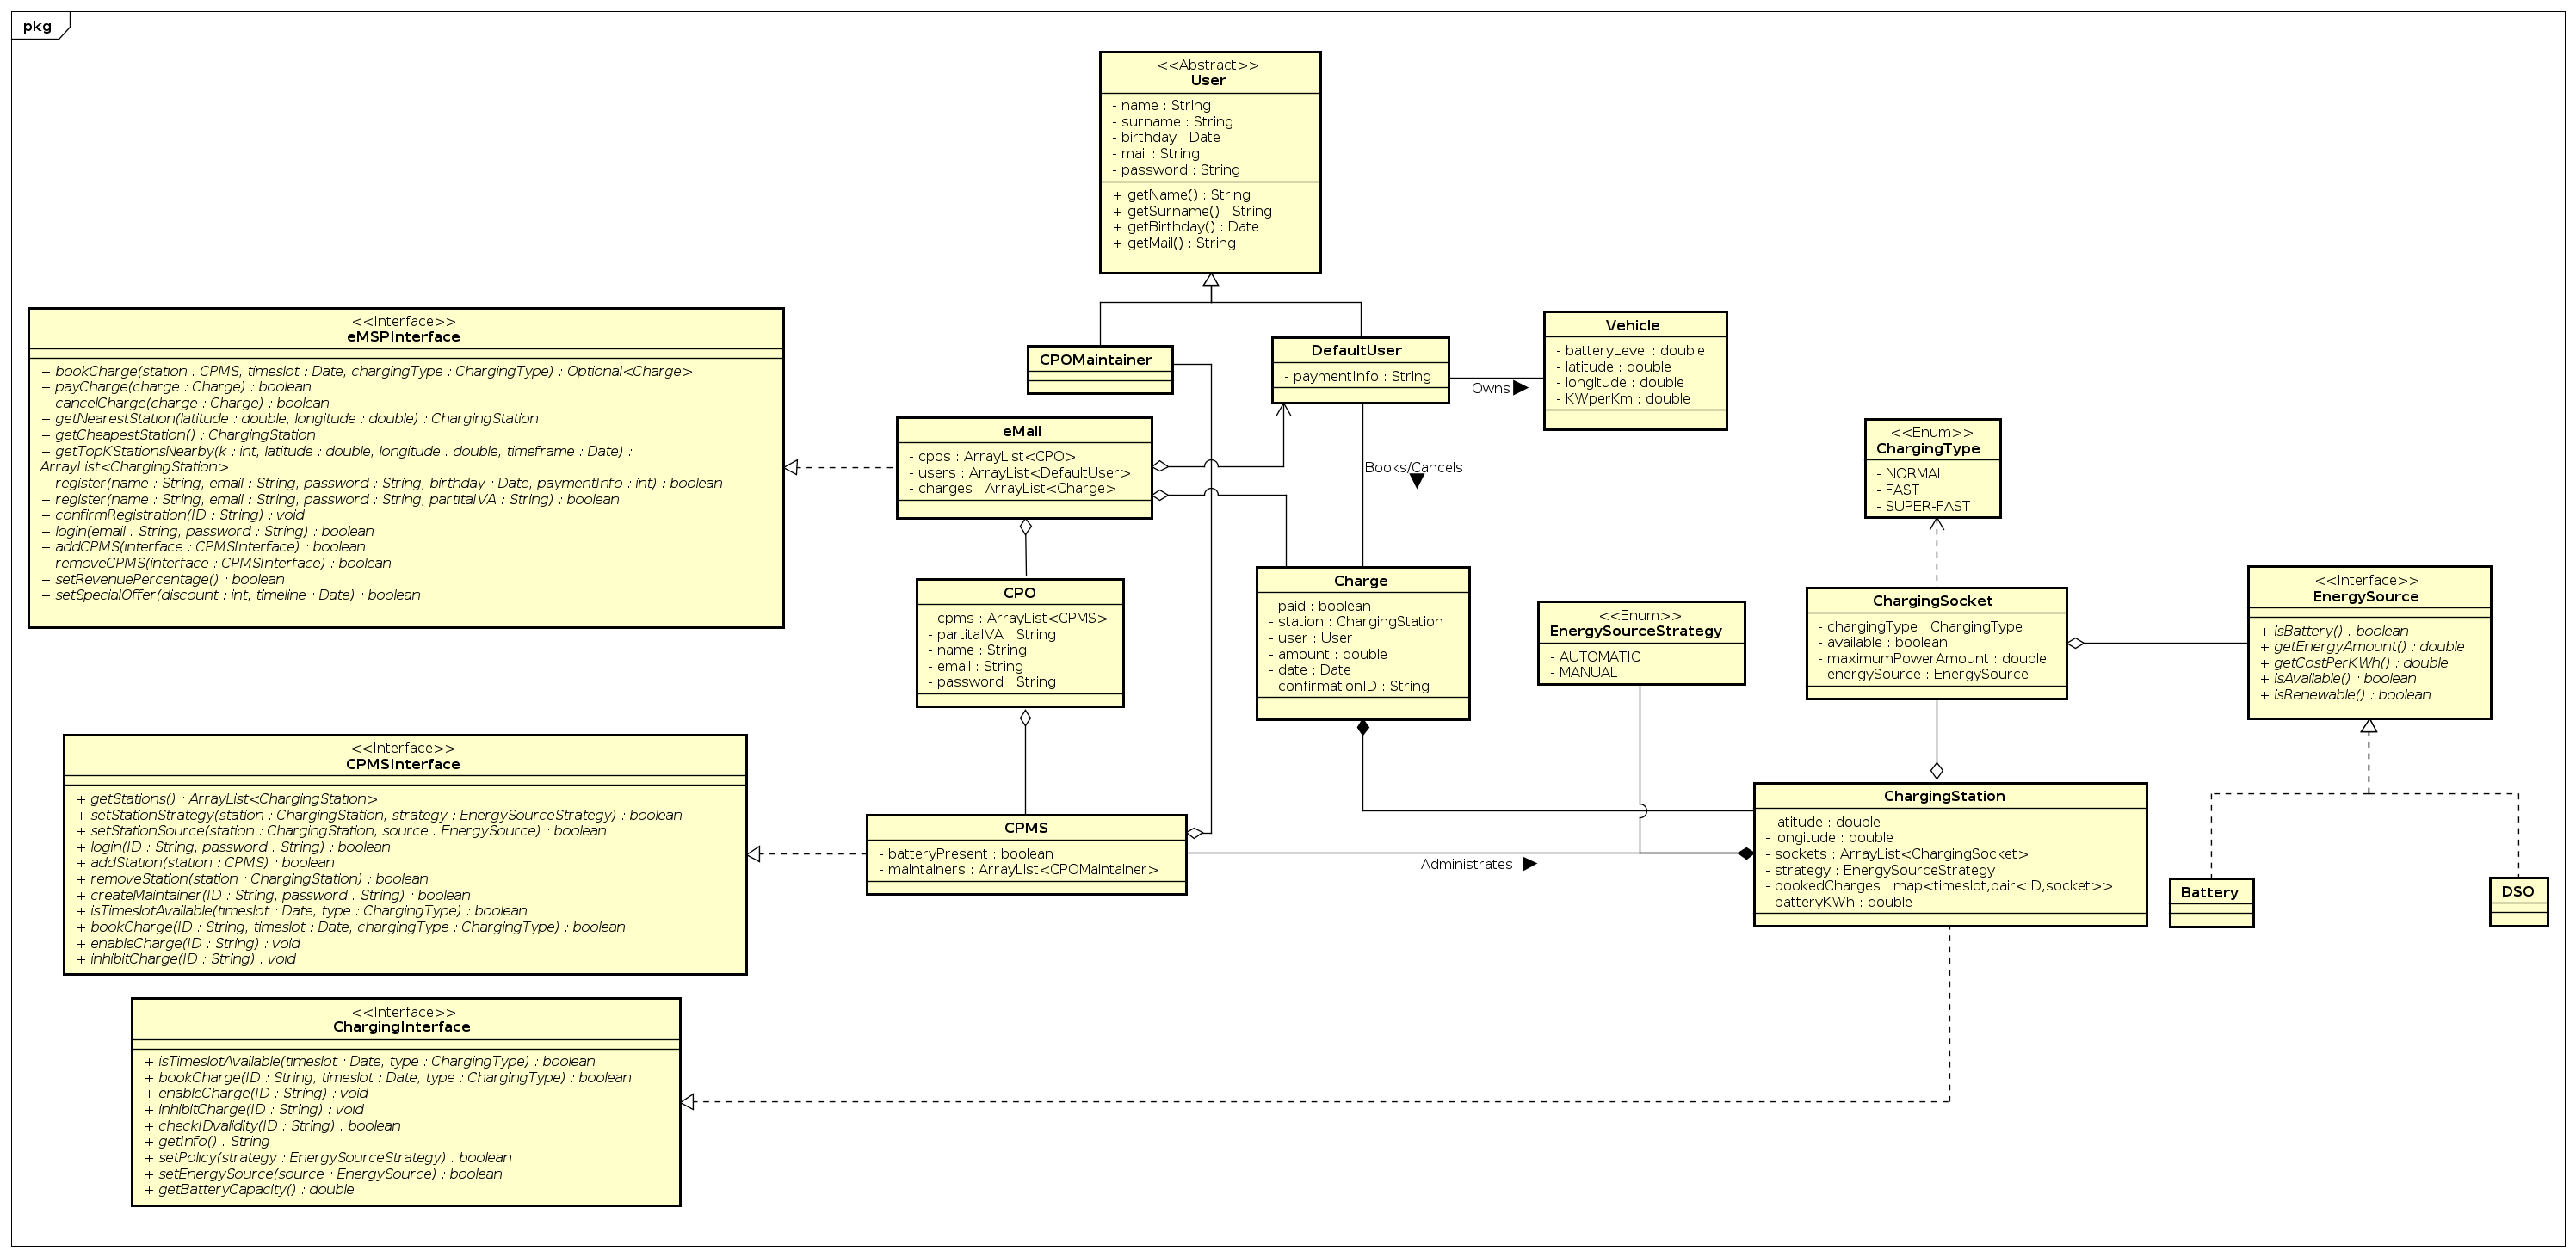
\includegraphics[keepaspectratio, width=16cm]{UML.png}
            \caption{UML}
      \end{center}
\end{figure}

\subsubsection{Scenarios}
\begin{enumerate}[label=S\arabic*]
      \item User Signs up:\\
            Lucy, wanting to use the system, opens the app, she is prompted to login or register,
            she chooses to register herself and inserts her personal info (email, password, payment information);
            an email is sent with a link to confirm the activation of the account, if the link is clicked within
            the first 15 minutes the account is activated and the sign up is successful,
            otherwise it is considered failed and the process must be repeated.
      \item User Logs in:\\
            Jay, after signing up, opens the app and he is prompted to insert his email and password,
            if the given information are correct the login is successful and he obtain access to his account
            and the service of the apps, otherwise the login is unsuccessful and it must be repeated.
      \item User searches for stations:\\
            Robert, once logged in, inserts the location and the time frame to search for charging stations.
            Once submitted a list of available charging station is displayed, the list is ordered by the distance of the station
            from the desired location. Via a menu Robert can choose to order the station either via distance or price,
            or to display unavailable station and set the maximum distance from the chosen location.
            Robert chooses a station obtaining more detailed information.
      \item User books a charge:\\
            Jessica, after choosing a station, decides to book it, the station location and booked time frame are displayed
            and she is asked to confirm the booking via a popup. Jessica then receives a confirmation email with the details
            of the charge (Location, time frame, socket id) and a confirmation pin to insert at the station.
      \item User charges the car:\\
            Mary, after booking a charge, arrives at the station, she parks her car at the designed socket
            and plugs her car in, Mary then inserts the confirmation pin in the socket to start the charge.
            The socket displays on a monitor the status and the finishing time of the charge.
            Once the charge is finished Mary receives a notification of finished charge,
            she gets her car and complete the charge.
      \item User gets charging suggestion based on his calendar:\\
            Josh is a very busy man, is also an avid google calendar user,
            setting up every event with correct time and locations.
            The service accessing his calendar finds the closest available charging station to each car movement,
            it estimates the battery level trough the gps data and once the battery is below fifty percent Josh gets notified
            about the possibility to charge his car.
            Josh liking the idea open the app and confirms the booking.
      \item Cpo subscribes to the system:\\
            Judy, the CEO of a famous CPO, wants to subscribe it to EMAll to improve sales and to access the CPMS feature.
            She opens a Website and select to sign up, she inserts the name, partita iva, a master password and the stations of the CPO.
            For each station she has to insert the number of charging port, the presence of batteries and, if there are any,
            wether to use the CPMS automatic source selector or to choose the preferred energy source.
      \item Cpo updates info about its system:\\
            The sysadmin of a CPO, Andy, after logging in with the master password has access to his CPO.
            Here he can change the number of stations, for each station he can update the number of socket and the energy source.
            He can also create and update maintainer account inserting the ID and password. For each maintainer he can choose which station the maintainer can maintain.
      \item Cpo employee logs in the service:\\
            Brett a CPO employee wants to access the service, he connects to the site and inserts the ID
            and password, if correct he logs in; otherwise the procedure fails and must be repeated.
      \item Maintainer maintains his assigned stations\\
            Lisa, a maintainer at a cpo logs in the service, here she can see the info of each station assigned to her.
            For each station she can: check the status(functioning or not), choose the energy source, update the number of available sockets.
            She can monitor the consumes, profitability and the usage of a specified station.
\end{enumerate}

\subsection{Product functions}
In the following subsections the functions of each subsystem are described.

\todo[inline]{Secondo me questi dovrebbero rispecchiare i metodi delle interfacce che si vedono nell'UML.}

\subsubsection{\ac{eMSP}}
\paragraph{Registering to the \ac{eMSP} as customer}
\paragraph{Logging to the \ac{eMSP} as customer}
\paragraph{Book a charge}

\paragraph{Cancel a charge}

\paragraph{Start a charge}
\todo[inline]{What about this point? Get information through the app about the starting of the charging process?}

\paragraph{Get nearest station}

\paragraph{Get cheapest station nearby}

\paragraph{Get top K stations nearby in base of characteristics}
\paragraph{Get infos about parcticular charging station}
number of charging sockets available, their type such as slow/fast/rapid, their cost, and, if all sockets of a certain type are occupied, the estimated amount of time until the first socket of that type is freed

\paragraph{Notify the user about the finish of the charge}

\paragraph{Pay for the obtained charge}

\paragraph{proactively suggest the user to go and charge the vehicle}
depending on the status of the
battery, the schedule of the user (this implies that the eMSP application can get access to the
calendar of the user and his/her navigation system), the special offers made available by some
CPOs, and the availability of charging slots at the identified stations

\subsubsection{\ac{CPMS}}
\paragraph{Registering to the \ac{CPMS} as \ac{CPO}}
\paragraph{Logging to the \ac{CPMS} as \ac{CPO}}
\paragraph{Choose manually to use the batteries}
\paragraph{Choose manually to use the \acp{DSO} energy}
\paragraph{Choose to make the \ac{CPMS} choose the energy source automatically}
\paragraph{Providing charging station informations for utilizators}
\paragraph{Providing charging station informations for maintainers}
\paragraph{Acquire informations about \acp{DSO}}
price



\subsection{User characteristics}

\subsection{Assumptions dependencies and constraints}
\subsubsection{Assumptions}
\begin{enumerate}[label=DA\arabic*]
      \item Users insert genuine data in the forms
      \item Users(Including CPOs) do not use the system with malicious intent
      \item Forse cancellare i booking
      \item All the electric vehicles can be charged by all the stations (no incompatibility)
      \item All the user have an active connection always available while using the service
\end{enumerate}
\clearpage